During the study, basic information about each participant was collected,
including their gender, age group, academic level, years of industry and
academic experience, regularity of working with microservices, the duration of
their experience with microservices, and the number of monoliths they have
assisted in decomposing.

Notably, the collected data indicates that 100\% of the participants in the
study were male, with the age distribution observed in
\Cref{fig:subjects_age_distribution}.

\begin{figure*}[!htb] \caption{Subjects Age Distribution}
  \label{fig:subjects_age_distribution} \centering
  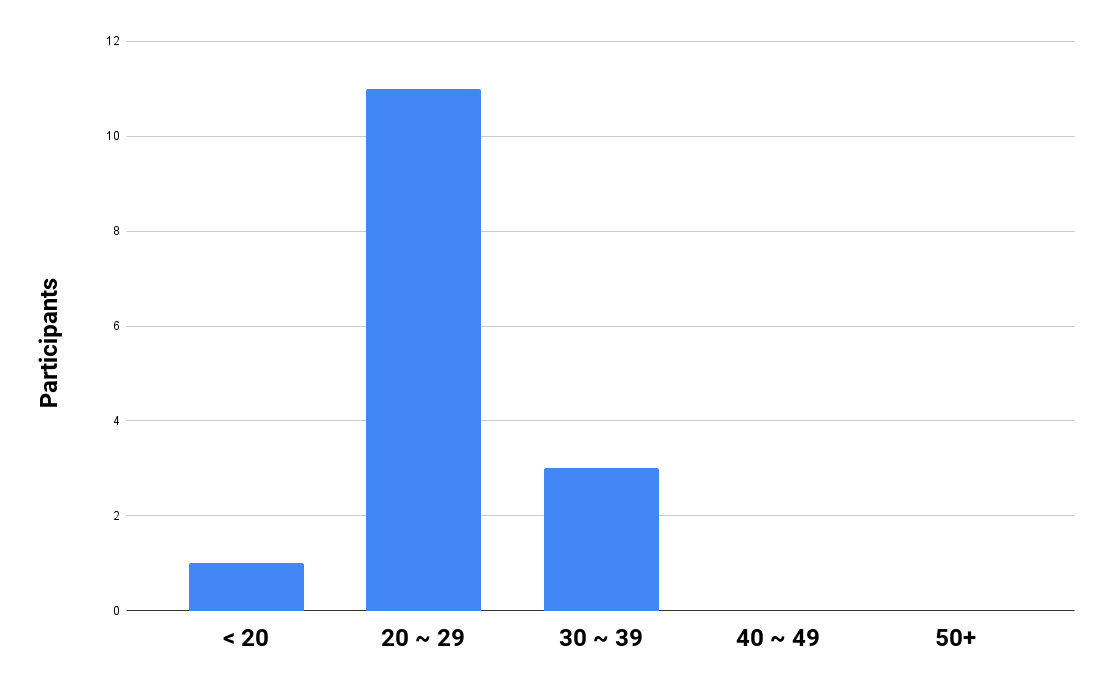
\includegraphics[width=\textwidth]{age_group}
\end{figure*}

The distribution of years of experience, considering both industry and academic
realms, can be found in \Cref{fig:year_experience_distribution}, and by
examining this distribution, it is possible to identify individuals with
wide industry experience, academic expertise, or a combination of both. This
differentiation is vital to understand the varied perspectives and knowledge
participants bring to the study. It also aids in analysing how their
backgrounds and experience may influence their perceptions, evaluations, and
performance during the decomposition tasks.

\begin{figure*}[!htb] \caption{Years of Experience Distribution}
  \label{fig:year_experience_distribution} \centering
  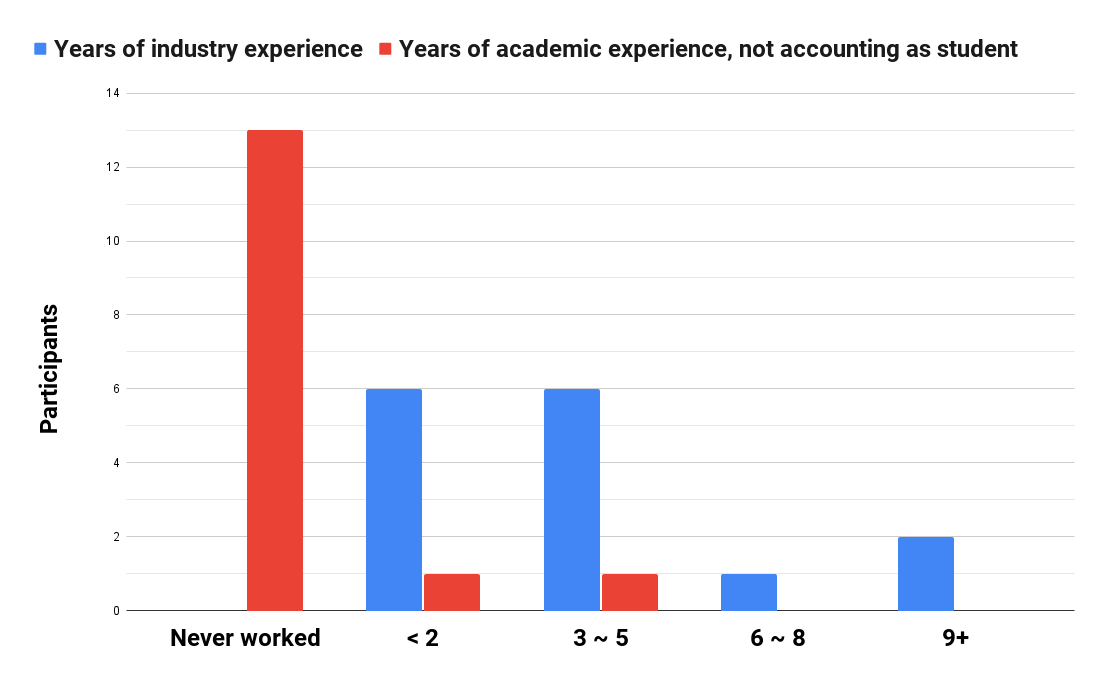
\includegraphics[width=\textwidth]{years_experience}
\end{figure*}

The study categorised their level of experience with microservices into four
categories: those who have never worked with microservices, those who have
worked with microservices at least once per month, those who have worked with
microservices at least once per week, and those who have worked with
microservices daily.

\Cref{fig:work_with_microservices} provides a visualisation of the
participants' frequency of working with microservices in their professional
activities.

\begin{figure*}[!htb] \caption{Frequency of work related with microservices}
  \label{fig:work_with_microservices} \centering
  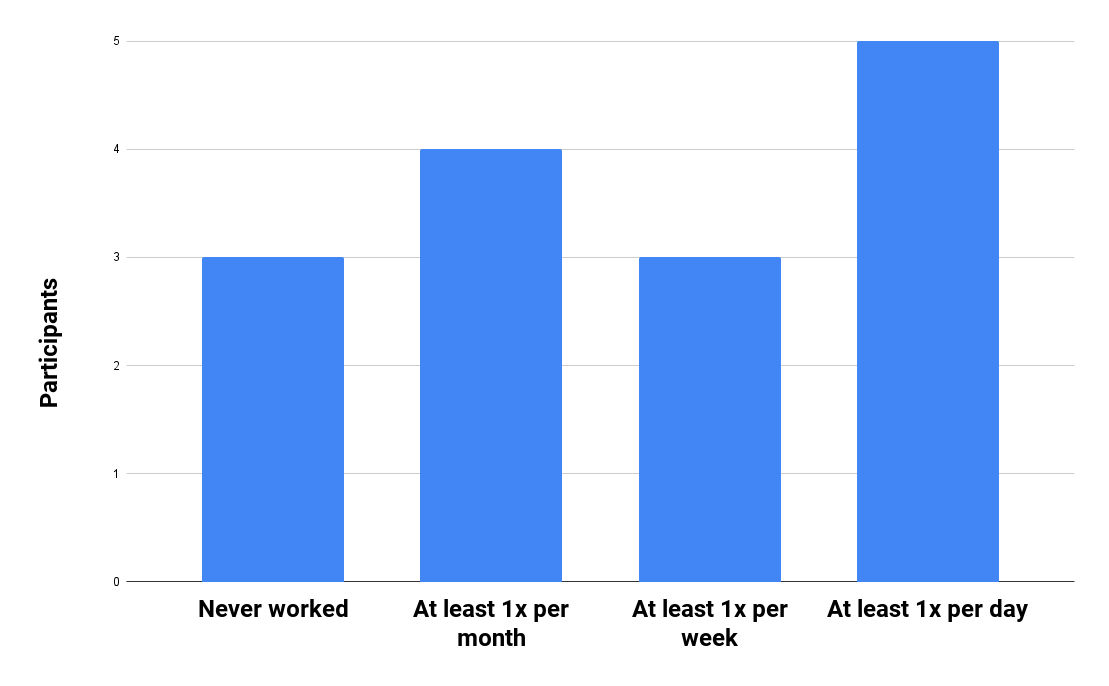
\includegraphics[width=\textwidth]{work_with_microservices}
\end{figure*}

The study also considered the participants' experience working with
microservices and the number of monolith decompositions they had undertaken, as
presented in \Cref{fig:years_working_microservices,fig:monoliths_decomposed}.

\begin{figure*}[!htb] \caption{Years working with microservices}
  \label{fig:years_working_microservices} \centering
  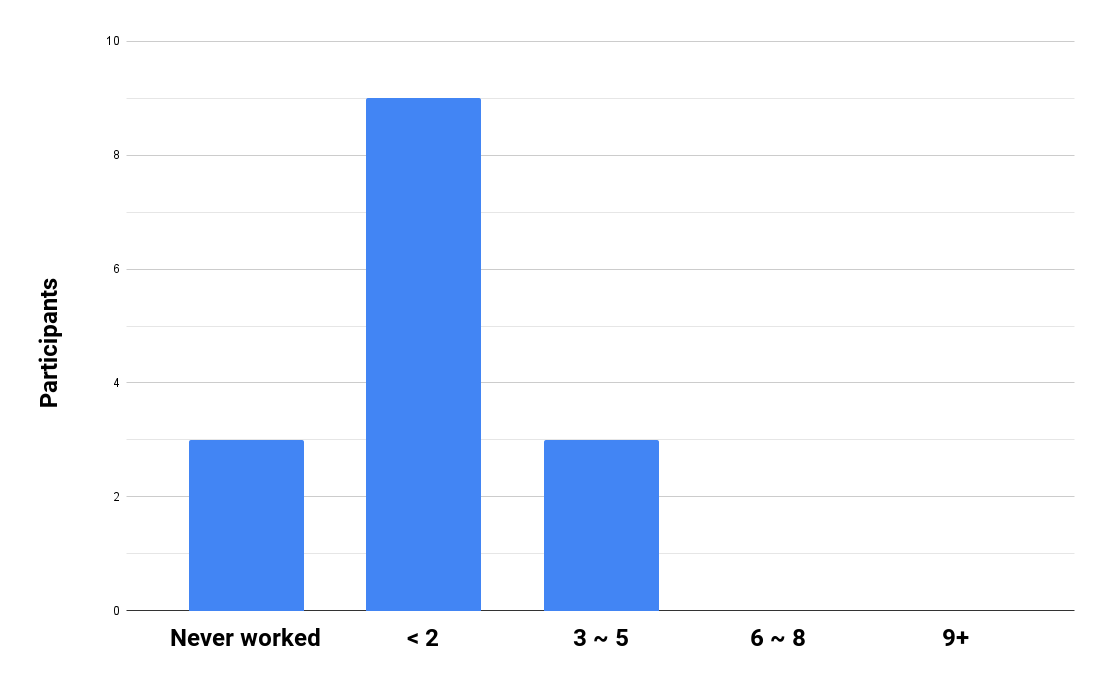
\includegraphics[width=\textwidth]{years_working_microservices}
\end{figure*}

\begin{figure*}[!htb] \caption{Amount of monoliths decomposed}
  \label{fig:monoliths_decomposed} \centering
  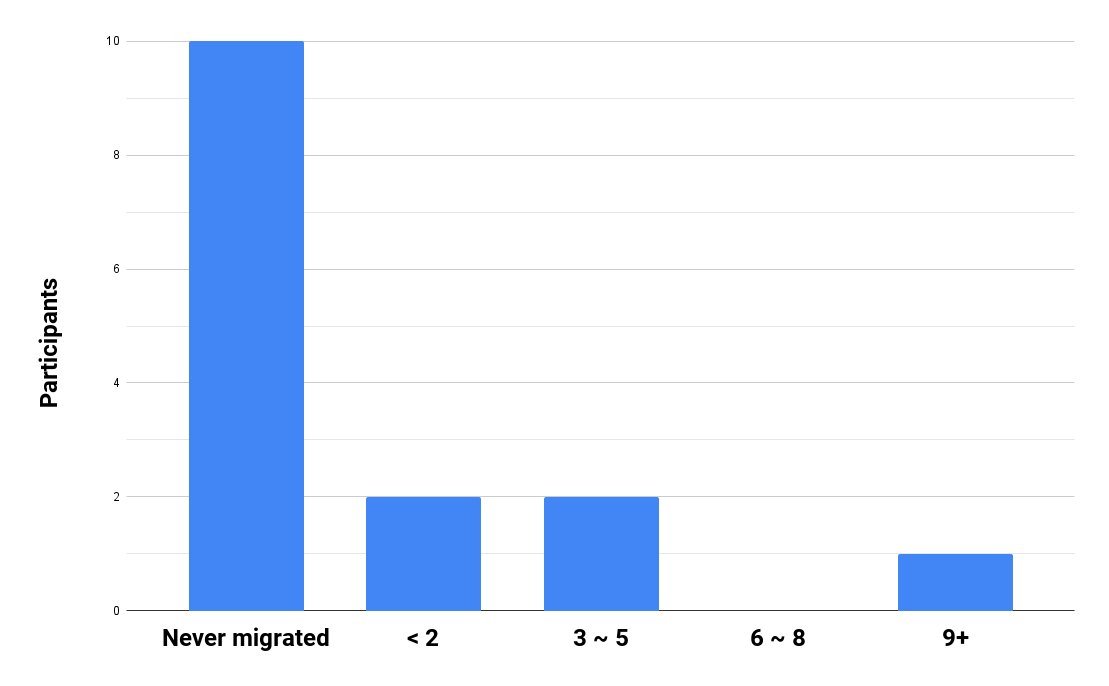
\includegraphics[width=\textwidth]{monoliths_decomposed}
\end{figure*}
